% This template contains modifications of the sfuthesis documentclass from Simon Fraser University.
% The new documentclass is bumrp (Brock University MRP)

% To compile in LaTeX you need to have the following files in the same directoty: template.tex, ref.bib, bumrp.cls

% The modifications were done by
% JF Lamarche
% Department of Economics, Brock University
% If you have questions or problems please contact him at jfl@brocku.ca

% The content is provided by Zain Virani, MBE student 2019.


\documentclass[undefended]{bumrp}

% Following lines are user dependent: lines 18 to 35

\title{Labour Market Polarization in Canada: To What Degree is Automation Responsible?}
\author{Zachary Mesic}
\previousdegrees{%
	B.A.,  Brock University,  2019}
\degree{Master of Business Economics}
\discipline{Economics}
\department{Department of Economics}
\faculty{Faculty of Graduate Studies}
\copyrightyear{2021}       % Year of submission
\semester{Summer 2021}     % term of submission
\date{September 10,  2021}     % obtain date from GPD

\keywords{automation, polarization, Routine-Biased Technological Change, Routine Task Intensity, offshoring, employment, wages, occupations.} % 3 to 5 keywords describing your MRP

\committee{
	\member{Miguel Cardoso}{Supervisor\\Assistant Professor \hspace{0.5cm}\rule{6cm}{0.01cm}}
	\member{Andrew Dickens}{Second Reader\\Assistant Professor \hspace{0.5cm}\rule{6cm}{0.01cm}}  % Could be a Co-Supervisor instead of Second Reader 

}



%   PACKAGES %%%%%%%%%%%%%%%%%%%%%%%%%%%%%%%%%%%%%%%%%%%%%%%%%%%%%%%%%%%%%%%%%%
%
%   Add any packages you need for your MRP here.
%   You don't need to call the following packages, which are already called in the bumrp class file:
%
%   - appendix
%   - etoolbox
%   - fontenc
%   - geometry
%   - lmodern
%   - nowidow
%   - setspace
%   - tocloft
%
%
%   The following packages are a few suggestions you might find useful.
%   (1) amsmath and amssymb are essential if you have math in your thesis; they provide useful commands like `blackboard bold'' symbols and environments for aligning equations.
%   (2) amsthm includes allows you to easily change the style and numbering of theorems. It also provides an environment for proofs.
%   (3) graphicx allows you to add images with \includegraphics{filename}.
%   (4) hyperref turns your citations and cross-references into clickable links, and adds metadata to the compiled PDF.
%   (5) chngcntr changes to numbering of the footnote counter such that they do not reset to 1 after each chapter



\usepackage{amsmath}                            % (1)
\usepackage{amssymb}                            % (1)
\usepackage{amsthm}                             % (2)
\usepackage{graphicx}                           % (3)
\usepackage[pdfborder={0 0 0}]{hyperref}        % (4)
\usepackage[svgnames,table]{xcolor}
\hypersetup{colorlinks,linkcolor={NavyBlue},citecolor={NavyBlue},urlcolor={red}}
\usepackage{chngcntr}                           % (5)
\counterwithout{footnote}{chapter}              % (5)


% Additional packages

\usepackage{sansmathfonts}
\usepackage[T1]{fontenc}
\renewcommand*\familydefault{\sfdefault}
\usepackage{threeparttable}
\usepackage{longtable}
\usepackage[utf8]{inputenc}
\usepackage{booktabs}
\usepackage{verbatim}
\usepackage{listings}
\usepackage{tabularx}
\usepackage[round, sort, compress, authoryear]{natbib}
\usepackage[italian,english]{babel}
\usepackage[autostyle]{csquotes}  
\usepackage{lscape}
\usepackage{hanging}

%   Spacing

%   (1) Use a single word space between sentences. If you disable this, you will have to manually control spacing around abbreviations.
%   (2) Correct the capitalization of "Chapter" and "Section" if you use the \autoref macro from the `hyperref` package.
%   (3) The LaTeX thesis template defaults to one-and-a-half line spacing. If your supervisor prefers double-spacing, you can redefine the \defaultspacing command.
%

\frenchspacing                                    % (1)
\renewcommand*{\chapterautorefname}{Chapter}      % (2)
\renewcommand*{\sectionautorefname}{Section}      % (2)
\renewcommand*{\subsectionautorefname}{Section}   % (2)
% \renewcommand{\defaultspacing}{\doublespacing}  % (3)



%   FRONTMATTER  %%%%%%%%%%%%%%%%%%%%%%%%%%%%%%%%%%%%%%%%%%%%%%%%%
%
%   Title page, committee page, copyright declaration, abstract, dedication, acknowledgements, table of contents, etc.
%

\begin{document}

\frontmatter
\maketitle{}
\makecommittee{}

\begin{Agreement}
In presenting this major research paper in partial fulfillment of the requirements for an advanced degree at Brock University, I agree that the Department of Economics shall have a right to make it freely available for reference and study.  I further agree that permission for extensive copying of this research for scholarly purposes may be granted by the Graduate Program Director of the Master of Business Economics program or by his or her representatives.  It is understood that copying or publication of the major research paper for financial gain shall not be allowed without my written permission.

\vspace{2cm}

\noindent
Department of Economics\\
\noindent Brock University\\
\noindent 1812 Sir Isaac Brock Way\\
\noindent St. Catharines, Ontario\\
\noindent L2S 3A1 CANADA

\vspace{2cm}
%%%%%%%%%%%%%%%%%%%%%
%Enter today's date
%%%%%%%%%%%%%%%%%%%%%
\noindent Signature:\hspace{0.5cm}\rule{6cm}{0.01cm}\hfill Date:\hspace{0.5cm}\rule{4cm}{0.01cm}

\end{Agreement}

\begin{abstract}
	In this paper, I investigate the pervasiveness of the Routine-Biased Technological Change (RBTC) model in explaining labour market polarization in Canada. I obtain average weekly employment and wage data from Statistics Canada’s Labour Force Survey (LFS) over the respective time periods 1987-2020 and 1997-2018. For this analysis, I rely on the 2011 version of the National Occupational Classification (NOC) to track 27 occupational categories. To measure the “routineness” or the relative amount of routine to manual and abstract task of occupations, I use the Routine Task Intensity (RTI) index. Alongside the RTI index, I use the “offshorability” index to measure an occupation’s susceptibility to offshoring. I find that Routine-Biased Technological Change does not fully explain labour market polarization in Canada. There are other factors, such as the resource boom outline in Green and Sand (2015), that may also responsible for polarization of the Canadian labour market.
\end{abstract}



\addtoToC{Table of Contents}%
\tableofcontents%
\clearpage

\addtoToC{List of Tables}%
\listoftables%
\clearpage

\addtoToC{List of Figures}%
\listoffigures%
\clearpage


% Your MRP starts next

\mainmatter%

\chapter{Motivation}

It is without question that automation has and continues to significantly transform many aspects of our society, including the economy. History is replete with examples of how automation has created economy-wide disruption. For example, the Industrial Revolution paved the way for many tasks such as spinning and weaving initially completed by artisans to become automated, leading to widespread disruption (Mantoux, 1928) (Acemoglu and Restrepo, 2019). The consequences of this displacement led to the infamous Luddite riots of the early 19th century, where English textile labourers formed a radical coalition against the forces of automation, industrialization, and new technologies through protest and destruction of textile machinery (Mokyr, 1990) (Acemoglu and Restrepo, 2019). 

Today, the forces of automation can be seen through the disruption of production-based jobs by automation technologies such as industrial robots and machinery (Graetz and Michaels 2018; Acemoglu and Restrepo 2018; Acemoglu and Restrepo, 2019). Specialized software and artificial intelligence have caused even those in white-collar positions in fields such as accounting, sales, logistics, trading, and managerial occupations to feel the impact of technology through the automation of tasks that they once performed (Acemoglu and Restrepo, 2019). 

One of the direct outcomes of automation’s impact on the economy is the phenomenon known as labour market polarization. Labour market polarization, in the context of this paper, is defined as the relative increase in labour demand for high-skill and low-skill occupations, accompanied by the relative decrease in labour demand for middle-skill occupations (Autor, Katz, and Kearney, 2006) (Goos and Manning, 2007). Growing patterns of labour market polarization have been documented across Western countries, including in the United States (Autor, Levy, and Murnane 2003; Autor, Katz, and Kearney 2006; Autor and Dorn 2013), Canada (Green and Sand, 2015), and Western Europe (Spitz-Oener 2006; Goos and Manning 2007; Dustmann, Ludsteck, and Schönberg 2009; Goos, Manning, and Salomons, 2014). 

Until recently, most studies relied on the “Skill-Biased Technological Change” (SBTC) model to explain labour market polarization, which suggests that “computerization” leads to an increase in the demand of college-educated workers and could explain rising wage inequalities (Autor, Katz, \& Kearney, 2006) (Goos, Manning, \& Salomons, 2014). Autor,  Levy,  and Murnane (2003) put forth an alternative understanding for how technology impacts labour markets, and how this impact could contribute to trends in labour market polarization. Goos, Manning, and Salomons (2014) refer to it as the “Routine-Biased Technological Change” (RBTC) model. The theory suggests that technological change decreases demand for routine and manual skills while increasing the demand for non-routine and cognitive skills.

Therefore, to further explore the causes of this phenomenon, I investigate the pervasiveness of the RBTC model in explaining labour market polarization in Canada. Given that the RBTC is the leading theory in explaining labour market polarization in other Western nations, it only stands to reason that RBTC may hold salience under a Canadian context. This is especially true when comparing Canada to the United States, as the two countries have many economic similarities. As far as I am aware, this is the first paper to investigate the causes of labour market polarization in Canada and thus the first to estimate the prevalence of RBTC in the country.

Labour market polarization has serious policy implications, including how to properly address societal issues such as income inequality. Since the 1970s, income inequality has increased significantly in most developed nations in the world (Partington, 2019). According to an analysis conducted by the Institute for Fiscal Studies (IFS), the share of income for the top 1\% of wealthiest households has almost tripled in the last four decades (Partington, 2019). In Canada, the fifth (or, highest) quintile was the only group to see an increase in its national income share over the period 1993 to 2008 (The Conference Board of Canada, 2021). Middle and low-income Canadians both saw decreases in their share of the national income (The Conference Board of Canada, 2021).

Rising inequality creates undesirable economic, social, and political outcomes (Qureshi, 2020). It has slowed economic growth by limiting aggregate demand and stifling growth in productivity. Some other consequences include social discontent, polarization in politics, and populist nationalism. It has also amplified societal and economic susceptibility to shocks, including the COVID-19 pandemic. Therefore, understanding what gives rise to labour market polarization, and by association inequality, is crucial to maintaining both economic and political stability. 

To date, much of the research has focused on the Unites States and little is known about the extent and causes of labour market polarization in Canada. Most of the current literature surrounding labour market polarization in Canada is concerned with identifying patterns and less about determining its causes. For example, Green and Sand (2015) find similar patterns of polarization in employment between Canada and the United States, but they do not offer an empirical model to determine the causes of the polarization in their paper.\footnote{Green and Sand (2015) point out that the model for technological change developed in the United States (the RBTC model) would not sufficiently explain labour market polarization in Canada. This is due to the lack of similarity in wage polarization trends between the US and Canada, specifically the fall in wages for low-paying occupations relative to middle and high-paying occupations. The resource boom experienced in Canada is more likely a cause for polarization in the country than technological change, according to the authors.} Therefore, this paper uses Canadian labour market data not only to observe patterns of polarization, but also to develop an empirical model that can test the origins of labour market polarization in the country.

I find that while there is some evidence in the data patterns that suggests that labour market polarization is caused by RBTC, there is not enough evidence provided in the empirical modelling which shows mixed results between RTI and hours worked in across occupations. It is likely that RBTC is not the sole, or even the primary contributor to labour market polarization in Canada, and that other factors such as the resource boom outlined in Green and Sand (2015) may also be responsible. Future researchers and policymakers therefore should consider explanations beyond RBTC when studying labour market polarization in the country.

This paper is outlined as follows. Chapter 2 provides a literature review, including background information on the Skill-Biased Technological Change (SBTC) model, the Routine-Biased Technological Change (RBTC) model, and the history and evidence of labour market polarization in Canada. Chapter 3 lists the sources of data that are used in the analysis, describes the variables of interest, and shows preliminary data patterns between the variables of interest and the employment and wage data. Chapter 4 outlines the methodology used in the empirical analysis. Chapter 5 discusses the results and main implications of the paper. Chapter 6 offers a conclusion to the findings and provides recommendations for future research into the topic.

\chapter{Background Information}

\section{Skill-Biased Technological Change}

Katz and Autor (1999) observe that disparities in the incomes across education and occupations slowed considerably throughout the 1970s across nearly every advanced country. However, since the end of the 1970s, there has been a deviation in the pattern in the development of the wage structure across education and occupation groups (Katz and Autor, 1999). Total inequality over wages and education has grown rapidly in countries such as the United States and the United Kingdom (Katz and Autor, 1999).

Katz and Autor (1999) find that the earnings of highly educated workers relative to those that are low-educated have grown significantly in the United States beginning in the 1950s. This is despite the growth that has been observed in the relative supply of highly educated workers (Katz and Autor, 1999). They claim that the increase in the relative demand for highly educated workers is crucial for understanding long-run wage structure evolution in the US, at least. According to the authors, Skill-Biased Technological Change is reflected by shifts in the industrial structure that occur from within-sector skill upgrading.

Tinbergen (1974, 1975) initially links the relative demand for skills to technology, characterizing technical change as ‘Skill-Biased’ (Acemoglu and Autor, 2010). More specifically, the theory suggests that returns experienced by skills and education are primarily due to the competition between the increase in the supply of labor market skills and technological change (Acemoglu and Autor, 2010). Technological change is considered skill biased because technological advancements tend to lead to an increase in the demand for more-skilled workers, including relatively educated workers (Acemoglu and Autor, 2010).

Observing the United States wage structure over the period of 1963 to 1987, Katz and Murphy (1992) come to similar conclusions as Katz and Autor (1999). They find that any observable changes in the wage structure and inequality in the U.S. can be accounted for by the ‘rapid secular growth’ in the relative demand for highly educated and highly skilled workers over the last 25 years. A significant portion of the relative shift in demand can be attributed to observable shifts in the employment arrangement of industrial and occupational to comparatively ‘skill-intensive’ sectors (Katz and Murphy, 1992). However, most of the shifts are occurring within ‘detailed’ sectors, a trend that reflects Skill-Biased Technological Change (Katz and Murphy, 1992).

According to the authors, there were two specific phenomena that occurred in the wage development of the United States that resulted in the relative increase of young college-educated men by approximately 30 percent over the period 1979 to 1987. The first was an increase in educational wage differentials, especially in the relative earnings of those who were college-educated. The second was an increase in the average wages of older workers relative to younger with comparatively lower education levels (Katz and Murphy, 1992).

Autor, Levy and Murnane (2003) argue that there is a consensus in the literature on the ‘strong association’ between computer adoption and the increased use of college-educated labor within detailed industries (Autor, Katz and Krueger, 1998; Berman, Bound and Griliches, 1994), within firms (Bresnahan, Brynjolfsson, and Hitt, 1999; Levy and Murnane, 1996), and across firms within industries Doms, Dunne, and Troske, 1997). Furthermore, these patterns of relative demand shift away from the lesser-educated to the higher-educated, which are likely brought on by computerization are observable not only in the U.S., but also in Canada (Gera, Gu, and Lin, 1999), across OECD countries (Machin and Van Reenan, 1998), and other developed nations (Berman, Bound and Machin, 1998) (Autor, Levy, and Murnane, 2003). 

\section{Routine-Biased Technological Change}

Autor, Levy, and Murnane (2003) put forth an alternative explanation for how technology impacts labour markets, and how this impact could contribute to trends in labour market polarization. They use worker samples taken from the Census and Current Population Survey (CPS) over the years of 1960-1998 and categorize occupations using the Dictionary of Occupational Titles, which offers descriptions of the skill requirements of jobs, and defines tasks as routine and non-routine cognitive and manual (Autor, Levy, and Murnane, 2003). 

Consistent with the literature, they find that over 1960-1998, there have been significant decreases in labour force participation in occupations that are relatively more routine task and routine manual task-intensive in the United States. This is accompanied by an increase in labour force participation in occupations that are relatively non-routine cognitive task-intensive, attributing ‘within-industry shifts’ in trends of employment that began in the 1970s as the reason for these broader trends (Autor, Levy, and Murnane, 2003).

In Autor and Dorn (2013), the authors analyze the potential causes of the growth in employment and wage polarization over the course of 1985-2005 in the United States. They hypothesize that employment and wage polarization is caused mainly by the interaction between consumer preferences and the automation of routine tasks. They apply a spatial equilibrium model which implies that there are varying levels of specialization among local labour markets in industries that are predominantly routine. 

To test their hypothesis of unbalanced technological progress, Autor and Dorn (2013) use data from 722 Commuting Zones in the United States which serve as proxies for localized labour markets. They find that commuting zones that were initially more routine-intensive saw a larger decrease in the share of routine-intensive occupations.\footnote{Important to note, the authors also test several alternative explanations for labour market polarization, including task offshoring, income and substitution effects in high-skill consumption and supply of labor, and demographic and economic shocks such as immigration, aging of population, entry of the female labor force, and decreases in manufacturing jobs. While there is some evidence for the significance of some of these variables, the authors conclude that none of them seemed to have been a major factor.} Additionally, the authors find that commuting zones that are proportionally more routine-intensive will adopt information technology due to falling prices and, consequently, displace labour from routine tasks.

Autor, Katz and Kearney (2006) observe changes in the US wage structure at the end of the 20th century and find evidence of polarization occurring at the higher and lower ends of the wage distribution. While inequality in wages among the top half of earners has been increasing since the 1980s, growth among the bottom half of earners has stalled. Contrary to the 1980s, the 1990s witnessed much greater increases in employment for those at the top and the bottom of the skill distribution in comparison to those in the middle.

To rationalize these findings, Autor et al. (2006) deploy a ‘model of computerization’, where the adoption of computer technologies results in: 1) the growth in employment across occupations that are non-routine cognitive task-intensive, 2) the decline in employment across occupations that are routine task-intensive, and 3) a minimal impact on occupations that are nonroutine manual task-intensive. They conclude that the model sufficiently explains patterns of polarization occurring in the US labour market.

Goos and Manning (2007) show that the United Kingdom has demonstrated labour market polarization patterns since 1975, given the relative increases in employment among the highest and lowest paid occupations. They find their results to be more consistent with the ‘routinization’ hypothesis put forward by Autor, Levy, and Murnane (2003) than the Skill-Biased Technological Change in characterizing technology’s impact on the labour market (although other factors are potentially important as well). Furthermore, they find that approximately one third of the increase in the log wage differentials between the 50th and 10th percentile and one-half of the increase in the 90th and 50th percentile of wage earners can be explained by labour market polarization.

Applying the Autor, Levy, and Murnane (2003) model to German wage data,  Dustmann, Ludsteck, and Schönberg (2009) show that there has been a rise in inequality since the 1980s. Increases were experienced more greatly by those at the top of the wage distribution throughout the 1980s, whereas the 1990s saw increases at both the top and bottom ends of the wage distribution relative to the middle (Dustmann, Ludsteck, and Schönberg, 2009). Spitz-Oener (2006) documents similar shifts in skill requirements in Germany over the period 1978-1998/99, with the largest increases in labour demand occurring at the bottom and top of the skills distribution. Both of their findings are consistent with the Autor, Levy, and Murnane (2003) model, which suggests that technological change is responsible for growing patterns in wage polarization.

Goos, Manning, and Salomons (2014) investigate the degree to which labour markets have polarized in 14 Western European countries over the 1993-2010 time period. They hypothesize that technological change that favours the replacement of labour involving routine tasks, which they refer to as Routine-Biased Technological Change (RBTC), along with the offshoring of tasks (it too moderately affected by technological change), can explain labour market polarization. Both RBTC and task offshoring cause the demand for middle-skill occupations to fall relative to the higher and lower ends of the skills distribution (Autor, Levy, and Murnane 2003; Autor, Katz, and Kearney 2006, 2008; Goos and Manning, 2007, 2014; Autor and Dorn 2013).

	They conclude that there is a shift in relative demand away from routine and offshorable occupations, with the routineness (or RBTC) of an occupation being a more important factor. Furthermore, they show that the model has important implications for between and within-industry components, in addition to sufficiently explaining ‘overall’ labour market polarization. Within-industry labour market polarization occurs when labour from within individual industries shifts away from routine occupations, but substantial shifts in labour between industries can also occur because of RBTC (Goos, Manning, and Salomons, 2014). 

\section{Evidence of Polarization in Canada}

There has been little research done on the causes of labour market polarization in Canada. One important exception is, Green and Sand (2015) who use Census and Labour Force Survey (LFS) data to analyze employment and wage structures in Canada over the period 1971-2012 to document labour market polarization. They find that prior to 1982, there is evidence of polarization, as employment in both higher and lower paying occupations increased more quickly than middle-paying occupations. However, before 2005, patterns in wage structure development more accurately reflect trends in inequality than in polarization (Green and Sand, 2015). This is due to high-paying occupations experiencing larger gains than middle-paying occupations, and middle-paying occupations experiencing larger gains than lower-paying occupations (Green and Sand, 2015).

\begin{figure}
    \centering
  \textbf{\caption{Change in Total Income by Income Percentile}}
    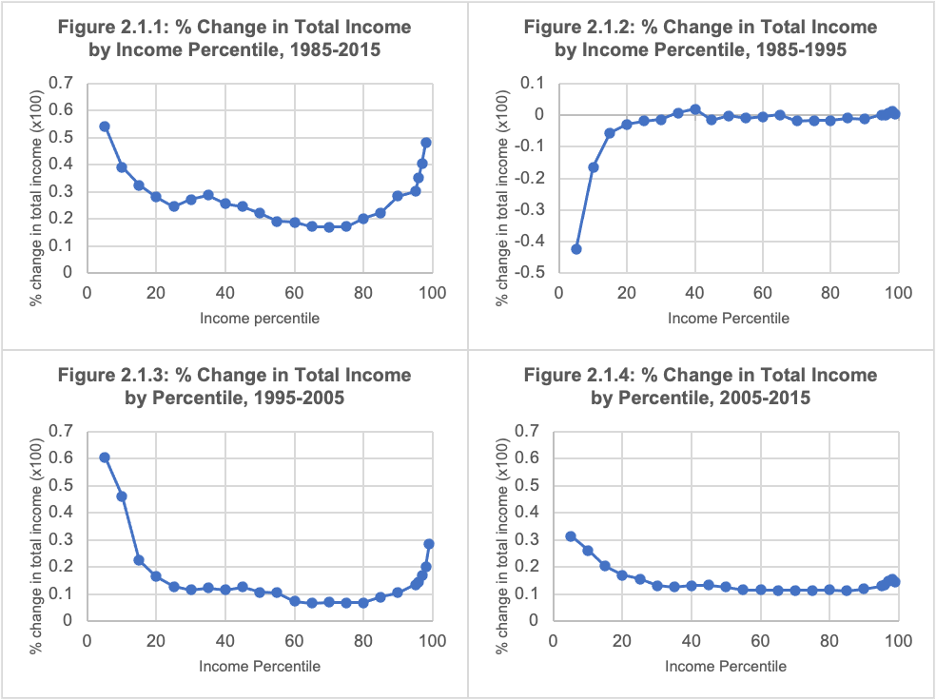
\includegraphics[scale=1]{figure21.png}
\begin{flushleft}
\textbf{Figure 2.1}: The above figure documents the percentage changes in total income by percentile from the years 1985, 1995, 2005, and 2015. The percentiles increase by rank of 5 up until the 95th, 96th, 97th, 98th, and 99th income percentiles. The data are collected from Statistics Canada’s Census of Population. Dollar values are measured in terms of 2015 constant dollars.
\end{flushleft}
\end{figure}

Using data from Statistics Canada’s Census of Population, I provide strong evidence of market polarization trends occurring in total incomes across income percentiles in the country. Figure 2.1.1 displays the percentage change in total income by percentile over the aggregate period 1985-2015. We see that over this time, growth in total income occurred predominantly at the tail ends of the income distribution. For example, at the 10th and 99th income percentiles, total income increased by approximately 54.25\% and 48.04\%, respectively. The smallest increases in total income occurred across the 60th to 80th income percentiles, with total income increasing by only approximately 19.17\% at the 60th percentile. These results suggest that there is a strong polarization at the tail ends of the income distribution, with the smallest gains in total income occurring for middle-wage earners.

Figure 2.1.2 displays the percentage change in total income by percentile over the period 1985-1995. The results in Figure 2.1.2 are unique such that rather than the lower tail of the income distribution experiencing the largest increases, it now experiences the largest decreases, with the 5th percentile experiencing a decline in income of approximately -42.45\% over the period.\footnote{This pattern is in line with the findings of Green and Sand (2015) which find relative to the United States, wages fell more significantly for low-paying occupations relative to middle and high-paying occupations prior to 2000 during the 1980s and 90s.} Therefore, the results obtained over 1985-1995 do not appear to fit the narrative of labour market polarization given the absence of relative increases in income at the lower and higher tails of the income distribution. Rather, the results seem to indicate that labour market polarization in the country did not occur until approximately the mid-1990s, as indicated by Figure 1.3. 

Figure 2.1.3 displays the percentage change in total income by percentile over the period 1995-2005. We see a very similar distribution to Figure 2.1.1 occurring over this period, with the largest increases in total income occurring at the tail ends of the income distribution. For example, at the 5th and 99th percentiles over 1995-2005, total income increased by approximately 60.62\% and 28.66\%, respectively. The smallest increases in total income occurred over the 65th to 85th percentiles over this period, with the 65th percentile seeing an income increase of only 6.61\% over the decade. These results are in line with Figure 2.1.1 and imply a strong polarization occurring at the tail ends of the income distribution.

Lastly, Figure 2.1.4 displays the percentage change in total income by percentile over the period 2005-2015. The results in Figure 2.1.4 appear to be exceptional to the aggregate pattern displayed in Figure 2.1.1, such that the increases in income at the tail ends of the income distribution are very minimal, with larger increases occurring at the lower tail. For example, at the 5th and 98th income percentiles, total income increased by approximately 31.51\% and 15.64\%, respectively, while the 65th income percentile experienced an 11.38\% increase. Therefore, the results in Figure 2.1.4 show only mild patterns of labour market polarization. It appears that most of the labour market polarization that occurred in Canada happened largely over the 1990s, as indicated by Figure 2.1.3, and began to significantly decline after the 2000s.

These data show that while the largest relative gains in income went to those at the bottom and top of the income distribution, the largest absolute gains are had at the top of the income distribution. While in relative terms, the lowest earners saw their incomes rise by approximately by the same percentage, the 90th percentile earners and above earned much more when one considers the gains in absolute terms. For example, 10th percentile earners saw a 54.25\% rise in their income, or from \$4,503 to \$6,946 over 1985-2015. Over the same period, 99th percentile earners only saw a 48.04\% rise in their income, but their incomes rose from \$158,148 to \$234,130, representing a \$73,539 difference in income growth.

Overall, these data demonstrate that there is strong labour market polarization that can be observed in Canada, primarily during the mid-1990s and occurring into the early 2000s. In every period, except 1985-1995, we see varying degrees of polarization occurring at the tail ends of the income distribution, with Figures 2.1.1 and 2.1.3 showing strong trends of polarization. We see that the largest gains in income occurred mostly in low-income percentiles (below 25th), and high-income percentiles (above 90th). The smallest increases were experienced by middle-income percentiles in these intervals, approximately over the 60th-80th percentile range. Though there is some polarization occurring at the tail ends of the income distribution during 2005-2015, it is very minimal when compared to the previous decade and occurs predominantly at the lower tail. In sum, while the results obtained over 1985-1995 do not fit the narrative of labour market polarization, we see in aggregate a typical U-shape distribution of gains in income over 1985-2015, with most of the polarization occurring post-1980s, during the 1990s, and coming to a slow in the mid-2000s.

\chapter{Data}

\section{Employment and Wages}

 To categorize employment and wages across occupations that will be linked to Routine Task Intensity data, I will rely on the National Occupational Classification (NOC).\footnote{It may be useful to look at other classifications as well, such as the International Standard Classification for Occupations (ISCO) for further research.} Through its classification structure, the NOC organizes the wide-ranging activity of occupations in Canada for purposes of collection, analysis, and dissemination. It is used to provide data on occupations for information on labour markets and program administration related to employment. The NOC version used in this paper is the NOC 2011 version, which is the third review of the NOC system and the National Occupational Classification for Statistics (NOC-S). Using the NOC classification allows me to map a measure of routine tasks to occupations to track the employment and wage outcomes in the Canadian labour market.

The datasets for employment and wages are both sourced from Statistics Canada’s Labour Force Survey. The Labour Force Survey data are used to create typical labour market markers, for example, the unemployment rate, employment rate and the participation rate. The Labour Force Survey also offers estimates on employment by industry, occupation, public and private sector, hours worked and more. It also allows for cross-classification by a range of demographic traits. Estimates are produced not only for Canada, but also the provinces, the territories, and a variety of sub-provincial regions. For workers, data regarding wage rates, union status, job permanency and establishment size are additionally produced.

For employment, I use the Statistics Canada datafile, Actual hours worked by occupation, annual. It measures the average actual hours worked in the reference week at an employee’s main job. Data are available at both the provincial and national level, for both sexes, over the period 1987-2020. For wages, the dataset used, also from Statistics Canada, is the Employee wages by occupation, annual. These wage data measure the average weekly wage rate across Canada for both full and part-time employees,  both sexes, aged 15 years and over, from 1997 to 2018.\footnote{It may also be worth examining the impact of RTI and offshorability on full-time vs. part-time workers as well.}  Wages in the initial dataset are in current 2021 dollars. For the empirical analysis, the base year of 2010 is used, thus wages are deflated to 2010 dollars using the CPI available on the Bank of Canada’s website.

\section{Routine Task Intensity (RTI) and Offshorability}

The first key variable of interest is the “routineness” of occupations, or the impact of Routine-Biased Technological Change. Goos, Manning, and Salomons (2014) use the five Dictionary Occupational Titles (DOT) task measures originally created by Autor, Levy, and Murnane (2003) and collapse them into three task aggregates as done by Autor, Katz and Kearney (2006, 2008), Autor and Dorn (2013) and Autor, Dorn and Hanson (2015). They include the Manual task measure, the Routine task measure, and the Abstract task measure. The RTI index of an occupation is then calculated as the difference between the log of Routine tasks and the sum of the log of Abstract and the log of Manual tasks and is normalized to have mean zero and unit standard deviation across occupations.\footnote{There were some instances in the mapping where two or more ISCO codes would map to one or more NOC codes. This means that some NOC codes had two values for RTI and offshorability. For example, the 2008 ISCO codes 21 Science and engineering professionals and 31 Science and engineering associate professionals map to both the 21 Professional occupations in natural and applied sciences and 22 Technical occupations related to natural and applied sciences from the 2011 NOC classification. In these instances, the measures were averaged out between them, and the average RTI and offshorability measure was applied to all occupations in that category.}

Goos et. al (2014) perform several crosswalks to obtain the data (which is originally categorized under Census occupational classifications) into the ISCO1988 occupational categories they use. Statistics Canada lists several concordances between classifications which can be implemented to map the RTI index variables classified under the Census occupational classification from Autor et al. (2003) to the 2011 NOC occupational classification.\footnote{On their website, Stats Canada provides a concordance between ISCO2008 and NOC 2011 occupational classifications. The ISCO website also provides a concordance between the ISCO1988 and ISCO2008 occupational classifications. Therefore, the crosswalk can successfully be completed from the ISCO1988 occupational classification used by Goos et. al (2014) to the NOC occupational classification from 2011.}

To control for any correlation between RTI and offshoring, a measure of “offshorability” is also included in the model.\footnote{Measures are available at both the occupational and industry level.} The measures for this variable are taken from Blinder and Kreuger (2013). The authors construct three measures using the individual level Princeton Data Improvement Initiative (PDII) dataset: one self-reported, one inferred, and one externally coded. The externally coded measure is the preferred measure by the authors.\footnote{The externally coded measure depends on the decisions of external coders who determine the degree to which an occupation is offshorable from the worker’s summary of their tasks.}  This is the measure used by Goos et al. (2014) and the one adopted in this paper. It is initially mapped into the European occupation classification and normalized to have a mean zero and standard deviation of one.\footnote{The occupational classification used by the authors is the Standard Occupational Classification (SOC) by the Bureau of Labor Statistics. Concordances between the SOC and NOC are provided by Statistics Canada. Therefore, obtaining offshorability measures under the NOC classification was of little issue.}

\section{Data Patterns}

\subsection{Employment Shares by Occupation and Province}

\begin{table}[!htbp] \centering 
\tiny
  \textbf{\caption{Measures and Change in Employment Shares at the NOC Level, 1997-2018}}
  \label{} 
\begin{tabular}{p{0.35\textwidth}p{0.11\textwidth}p{0.11\textwidth}p{0.11\textwidth}p{0.11\textwidth}p{0.11\textwidth}}
\\[-1.8ex]\hline 
\hline \\[-1.8ex] 
 NOC & Mean Occupational Wage, 1997-2018 (1) & Average employment share, 1997 (in \%) (2)	& Percentage point change, 1997-2018 (3) & RTI (4) & Offshorability (5) \\
\hline \\[-1.8ex] 
\textit{High-paying occupations}	& &	\textbf{36.54}	& \textbf{-0.05}	& \textbf{-0.34} & \textbf{-0.04} \\
\\[-1.8ex]\hline 
\hline \\[-1.8ex] 
Professional occupations in natural and applied sciences [21]	& 1034.78 &	4.18	& -3.73 &	-0.61 &	0.47 \\
Occupations in front-line public protection services [43]	& 993.61	& 4.24 &	4.77	& -0.60	& -0.94 \\
Professional occupations in business and finance [11]	& 905.25	& 4.06	& -3.65 & -0.73 &	0.21 \\
Professional occupations in health (except nursing) [31]	& 887.51	& 4.13	& -1.77	& -0.67	& -0.76 \\
Professional occupations in law and social, community and government services [41]	& 884.79	& 4.07	& -5.70 &	-0.44	& 0.10 \\
Processing, manufacturing and utilities supervisors and central control operators [92]	& 840.75	& 4.35 & 	2.53 &	0.39	& 0.47 \\
Professional occupations in nursing [30]	& 811.54	& 3.28 &	8.79	& -0.67	& -0.76 \\
Technical occupations related to natural and applied sciences [22]	& 807.91	& 4.05	& -0.81	& -0.61	& 0.47 \\
Industrial, electrical and construction trades [72]	& 773.54 &	4.19	& 0.55	& 0.85	& 0.35 \\
\hline \\[-1.8ex] 
\textit{Middle-paying occupations}	& &	\textbf{34.42} &	\textbf{0.22}	 & \textbf{-0.41} & \textbf{0.00} \\
\\[-1.8ex]\hline 
\hline \\[-1.8ex] 
Transport and heavy equipment operation and related maintenance occupations [75]	& 640.09	& 4.41 &	-0.57 &	-1.50	& -1.00 \\
Technical occupations in health [32]	& 632.48	& 3.43	& -1.63	& -0.67	& -0.76 \\
Retail sales supervisors and specialized sales occupations [62]	& 628.39	& 4.22	& -6.66	& 0.05	& -0.89 \\
Administrative and financial supervisors and administrative occupations [12]	& 611.33	& 3.65	& 0.32	& -1.13 &	-0.48 \\
Assemblers in manufacturing [95]	& 583.05	& 4.14	& -1.00	& 0.49	& 2.35 \\
Trades helpers, construction labourers and related occupations [76]	& 579.49	& 3.99	& 2.31	& -0.19	& -0.93 \\
Finance, insurance and related business administrative occupations [13]	& 559.67	& 3.22	& 3.03	& -0.73 &	0.21 \\
Processing and manufacturing machine operators and related production workers [94]	& 552.07	& 4.05	& 3.09 &	0.39 	& 0.47 \\
Paraprofessional occupations in legal, social, community and education services [42]	& 492.53	& 3.32	& 4.59 &	-0.44	& 0.10 \\
\hline \\[-1.8ex] 
\textit{Low-paying occupations}	& &	\textbf{29.03}	& \textbf{-0.19} & \textbf{0.50} & \textbf{-0.22} \\
\\[-1.8ex]\hline 
\hline \\[-1.8ex] 
Office support occupations [14]	& 488.59	& 3.40 &	0.50	& 2.24	& 0.40 \\
Labourers in processing, manufacturing and utilities [96]	& 468.66	& 3.93	& 0.71	& 0.39	& 0.47 \\
Technical occupations in art, culture, recreation and sport [52]	& 468.59	& 3.42	& -8.40	& 1.59	& 1.66 \\
Assisting occupations in support of health services [34]	& 458.30	& 3.29	& 3.97	& -0.67	& -0.76 \\
Care providers and educational, legal and public protection support occupations [44]	 & 415.12	& 3.08	& 2.39 &	-0.60 &	-0.94 \\
Sales representatives and salespersons - wholesale and retail trade [64]	& 404.38	& 3.24	& 0.43	& 0.05 &	-0.89 \\
Service representatives and other customer and personal services occupations [65]	& 371.85	& 3.17	& -0.27 &	1.41	& -0.25 \\
Service support and other service occupations, n.e.c. [67]	& 308.62	& 2.90	& -0.85	& 0.03	& -0.81 \\
Sales support occupations [66]	& 230.85	& 2.60	& 0.02	& 0.05	& -0.89 \\
\hline 
\hline \\[-1.8ex]  
\end{tabular} 
\end{table} 

\newpage

\begin{flushleft}
\textbf{Table 3.1}: Column 1: occupations are ranked by their mean occupational wage across all years. Columns 2-3: the initial employment shares of occupations in the base year of 1997 and the percentage point changes across occupations over the period 1997-2018. Columns 4-5: measures of Routine Task Intensity (RTI) (Autor and Dorn, 2013) and offshorability (Blinder and Kreuger, 2013) of an occupation. A higher value indicates that an occupation is more routine-task intensive, or more offshorable, whereas a lower value indicates that an occupation is less routine-task intensive, or less offshorable. 
\end{flushleft}

The results in Table 3.1 do not seem to point toward any pattern of polarization in shares of employment. The average percentage point change in employment share is fairly similar for each of the three occupational categories over the period 1997-2018, with low and high-paying occupations seeing a net decline of -0.19\% and -0.05\%, respectively. Interestingly enough, middle-paying occupations actually saw a relative increase in their employment share of approximately 0.22\%.  This result does not appear to be in line with the RBTC theory, as middle-paying occupations, which are often considered more routine, should have seen a decline in their share of employment of the given period. 

Perhaps the reason middle-paying occupations saw the largest gains in employment is that they also possessed the most negative values of RTI on average and thus are less routine than high and low-paying occupations.\footnote{The correlation coefficient between the percentage change in employment shares and RTI is -0.22, which implies that the more routine an occupation is, the smaller its share of employment will be. This result is in line with the RBTC model.} The RTI of middle-paying occupations was approximately -0.41, while high and low-paying occupations had an RTI of  -0.34 and 0.50, respectively.  While the implied result is technically in line with the RBTC model, RBTC characterizes middle-paying occupations as being more routine. In Canada's case, it appears that the opposite is true, and that the routineness of a given occupation is not dependent on its wage or skill level.

This result could however simply be due to outliers. For example, \textit{Transport and heavy equipment operation and related maintenance occupations [75]} is the highest paid middle-paying occupation, and has an RTI of -1.50, while \textit{Industrial, electrical and construction trades [72]} is the lowest high-paying occupation, and has an RTI of approximately 0.85. Therefore, it is possible that the sample size of occupations needs to be increased in order to account for some of the skewed effects that the outliers are creating on the data.

\newpage

\begin{table}[!htbp] \centering 
\tiny
\textbf{\caption{Measures and Change in Employment Shares at the Provincial Level, 1997-2018}}
  \label{} 
\begin{tabular}{p{0.2\textwidth}p{0.09\textwidth}p{0.09\textwidth}p{0.09\textwidth}p{0.09\textwidth}p{0.09\textwidth}p{0.09\textwidth}}
\\[-1.8ex]\hline 
\hline \\[-1.8ex] 
& \multicolumn{2}{c}{\textbf{Low-paying occupations}} & \multicolumn{2}{c}{\textbf{Middle-paying occupations}} & \multicolumn{2}{c}{\textbf{High-paying occupations}}\\
\hline \\[-1.8ex] 
Province &	Employment Share in 1997 (in \%)	& \% point change (1997-2018) &	Employment Share in 1997 (in \%) & 	\% point change (1997-2018)	& Employment Share in 1997 (in \%)	& \% point change (1997-2018) \\
\hline \\[-1.8ex] 
 &	 &	\textbf{-0.05}  & 	& \textbf{2.14}	& 	&  \textbf{-1.44} \\
\hline \\[-1.8ex] 
Alberta	& 28.76	& 0.50	& 34.58	& -0.42	& 36.66	& 0.00 \\
British Columbia & 	29.57	& -0.03	& 33.56	& 1.47	& 36.87	& -1.32 \\
Manitoba	& 28.64 & 	0.29	& 34.05	& 2.67	& 37.31	& -2.67 \\
New Brunswick	& 29.59	& -1.27	& 34.26	& 2.65	& 36.15	& -1.47 \\
Newfoundland and Labrador	& 30.25	& -6.72	& 31.35	& 13.03	& 38.39 & 	-4.63 \\
Nova Scotia	& 28.94	& -0.10	& 34.53	& -0.17	& 36.53 & 	-0.52 \\
Ontario	& 28.65	& 0.56 & 	34.52	& -0.50	& 36.84	& 0.03 \\
Prince Edward Island	& 28.79	& 2.95	& 34.17	& 2.78	& 37.04	& -4.86 \\
Quebec	& 29.46	& -1.22	& 34.82	& 0.05	& 35.72	& 0.96 \\
Saskatchewan	& 28.75	& 0.05	& 34.81	& -0.17	& 36.44	& 0.12 \\
\hline 
\hline \\[-1.8ex]  
\end{tabular} 
\end{table} 

\begin{flushleft}
\textbf{Table 3.2}: The above table displays the average employment shares for low-paying, middle-paying, and high-paying occupations across provinces in 1997 and the percent point changes in employment shares over 1997-2018 for each occupational income group. 
\end{flushleft}

Motivated by Green and Sand (2015), Table 3.2 provides a provincial breakdown of employment shares in order to observe any polarization that may be occuring in wage categories across Canadian provinces. The results are similar to Table 3.1; on average, occupations that are considered middle-paying saw an increase in their employment share of 2.14\%, while occupations that are considered low and high-paying saw their employment shares fall by -0.05\% and -1.44\%, respectively.  It appears that the analysis on provincial employment shares does not reveal any additional evidence of labour market polarization in Canada.\footnote{Green and Sand (2015) cite Alberta as an example of a province experiencing labour market polarization due to the post-2000 resource boom. It appears that there is at least some evidence of this, as the employment share of middle-paying occupations in Alberta across 1997-2018 fell by approximately -0.42\%, while low-paying occupations increased by 0.5\%, and high-paying occupations did not change at all.}

\subsection{RTI and Offshorability vs. Total Employment and Wages}

In this section, I provide some preliminary data patterns to observe the relationship of our key variables with the employment and wage data. Figures 3.1.1 and 3.1.2 display scatterplots of the relationships between RTI and offshorability and the percentage point change in the average actual hours of occupations over the period 1997-2018. Both figures show that there is a negative relationship between the variables of interest and the percentage change in hours worked. The relationship is more strongly negative in the Figure 3.1.1 than in 3.1.2. A one-unit increase in the RTI index will lead to an approximate 1.12\% decrease in hours worked, whereas a one-point increase in the offshorability index will only result in an approximate 0.47\% decrease in hours worked. These results suggest that occupations that are more routine task-intensive and offshorable are more likely to see minimal decreases in average hours worked. 

Figures 3.1.3 and 3.1.4 display scatterplots of the relationships between RTI and offshorability and the percentage point change in the average weekly wage rate of occupations over the period 1997-2018. Like Figures 3.1.1 and 3.1.2, both figures show a negative relationship between the variables of interest and the percentage change in wages. Both relationships are more strongly negative, with a one-point increase in the RTI index resulting in an approximate 6.19\% decrease in wages and a one-point increase in the offshorability index resulting in an approximate 5.73\% decrease in wages. These results suggest that not only are occupations that are more routine task-intensive and offshorable more likely to see decreases in their wages and hours worked, with wages being more negatively affected.

\begin{figure}
    \centering
    \textbf{\caption{RTI and Offshorability vs. Change in Hours Worked and Weekly Wage Rate}}
    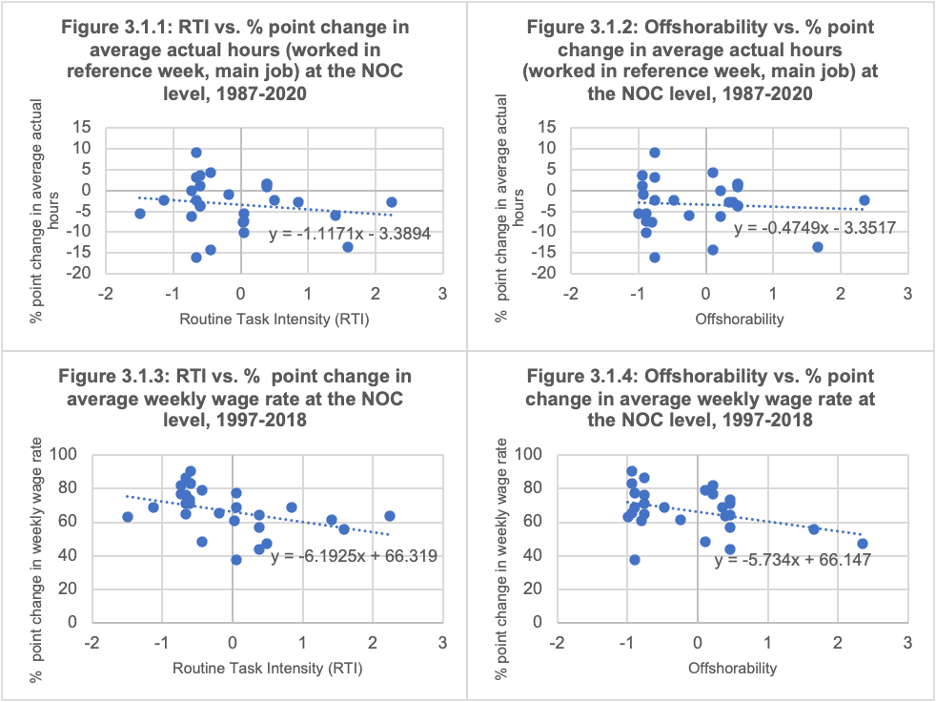
\includegraphics[scale=1]{figure31.png}
\begin{flushleft}
\textbf{Figure 3.1}: The above figure shows scatterplots of the relationship between the two variables of interest (RTI and Offshorability) and the percentage point change in the average number of hours worked and the wage rate in Canada. The employment data used are from Statistics Canada’s Labour Force Survey and is obtained over the period 1987-2020. The wage data also come from the LFS and are obtained over the period 1997-2018. 
\end{flushleft}
\end{figure}

For robustness, the standard errors are collected and used to determine the statistical significance of the estimations. Standard errors for Figures 3.1.1 and 3.1.2 are approximately 1.36 and 1.39, respectively. The t-statistics for Figures 3.1.1 and 3.1.2 are approximately 0.82 and 0.34, indicating that neither the estimate for the relationship between RTI and percentage change in hours worked nor Offshorability and percentage change in hours worked are statistically significant from zero at the 5\% level (t-statistic < 1.96). Standard errors for Figures 3.1.3 and 3.1.4 are 2.76 and 2.84, respectively. The t-statistics for Figures 3.1.3 and 3.1.4 are approximately 2.24 and 2.02, indicating that both the estimates for the relationship between RTI and percentage change in the weekly wage rate and Offshorability and percentage change in the weekly wage rate are statistically significant at the 5\% level (t-statistic > 1.96). 

\newpage

\subsection{RTI and Offshorability vs. Employment Share and Relative Wage}

Figures 3.2.1 and 3.2.2 display scatterplots of the relationships between RTI and offshorability and the percentage point change in the average employment share of occupations over the period 1997-2018. Both figures show that there is a negative relationship between the variables of interest and the percentage point change in employment share. This time, the relationship is more strongly negative in the Figure 3.2.2 than in 3.2.1. Whereas one-point increase in the RTI index will only result in an approximate 0.90\% decrease in employment share, a one-point increase in the offshorability index will result in an approximate 1.30\% decrease in employment share. These results support the previous findings that occupations that were more routine task-intensive and offshorable were more likely to see minimal decreases in average hours worked. 

Figures 3.2.3 and 3.2.4 display scatterplots of the relationships between RTI and offshorability and the percentage change in the relative wage of occupations over the period 1997-2018. Like Figures 3.2.1 and 3.2.2, both figures show a negative relationship between the variables of interest and the percentage point change in relative wage. Both relationships are strongly negative, with a one-point increase in the RTI index resulting in an approximate 3.69\% decrease in the relative wage and a one-point increase in the offshorability index resulting in an approximate 3.41\% decrease in the relative wage. 

\begin{figure}
    \centering
    \textbf{\caption{RTI and Offshorability vs. Change in Employment Share and Relative Wage}}
    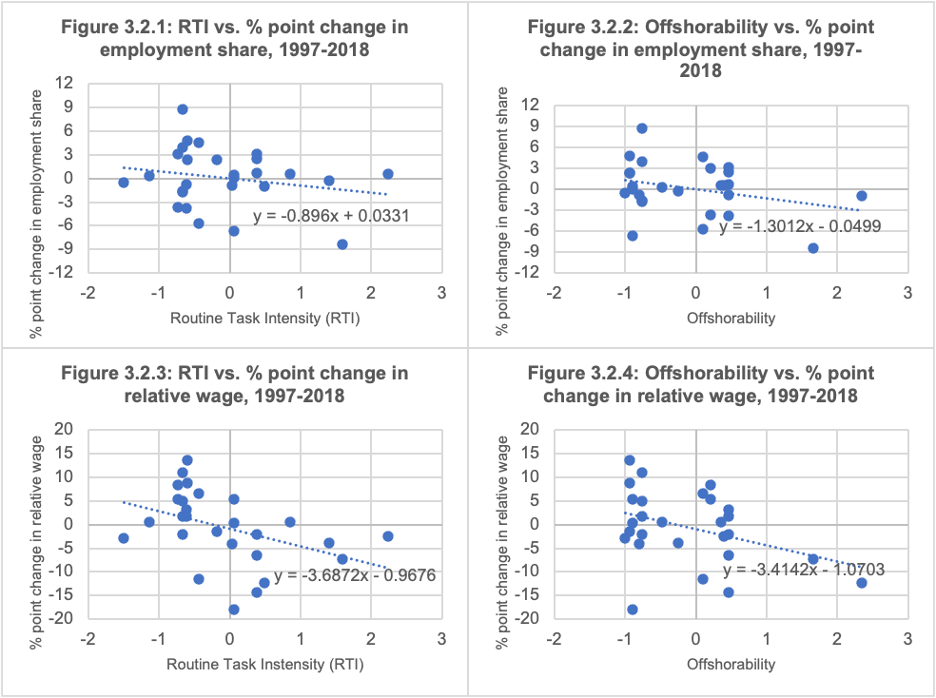
\includegraphics[scale=1]{figure32.png}
\begin{flushleft}
\textbf{Figure 3.2}: The above figure shows scatterplots of the relationship between the two variables of interest (RTI and Offshorability) and the percentage point change in the employment shares and relative wages of occupations over 1997-2018. The employment and wage data used are from Statistics Canada’s Labour Force Survey.
\end{flushleft}
\end{figure}

These results also support previous findings; the decreases in wages of occupations that are more routine task-intensive and offshorable are more significant than the decreases in employment or hours worked. Furthermore, the findings in Figure 3.2 show that the higher the RTI and offshorability index is, the more likely it is for labour to shift away from occupations that are more routine-intensive and offshorable to those that are less routine-intensive and offshorable. The results obtained in Figures 3.1 and 3.2 are both in line with the anticipated outcome of the RBTC model, which predicts a negative relationship between RTI and offshorability, and hours worked and the wage rate.

Once again, standard errors are collected and used to determine the statistical significance of the estimations. Standard errors for Figures 3.2.1 and 3.2.2 are approximately 0.85 and 0.84, respectively. The t-statistics for Figures 3.2.1 and 3.2.2 are approximately 1.06 and 1.55, indicating that neither the estimates for the relationship between RTI and percentage change in the employment share nor Offshorability and percentage change in the employment share are statistically significant from zero at the 5\% level (t-statistic < 1.96). Standard errors for Figures 3.2.3 and 3.2.4 are 1.64 and 1.69, respectively. The t-statistics for Figures 3.2.3 and 3.2.4 are approximately 2.24 and 2.02, indicating that both the estimates for the relationship between RTI and percentage change in the relative wage and Offshorability and percentage change in the relative wage are statistically significant at the 5\% level (t-statistic > 1.96).

\chapter{Methodology}

I use two main panel model regression specifications to test the relationship between RTI and offshorability and the employment outcomes of occupations in Canada. The first is a simple Pooled Ordinary Least-Squares (OLS) Regression Model, the second features two variations of the Fixed Effects Regression Model, which are the Least-Squares Dummy Variable Model and the One-way “Within” Fixed Effects Model.

\section{Pooled OLS Regression Model}

Consider the following simple Pooled OLS Regression Model:

\begin{center}
$$ Y_{ij,t} = \beta_{0} + \beta_{1} w_{ij,t} + \beta_{2} RTI_{i} + \beta_{3} Off_{i} + e_{ij,t} $$ (1)
\end{center}

where $Y_{ij,t}$ represents the average number of hours worked in the reference week at a worker’s main job, for occupation $i$ in province $j$ over time $t$ $\epsilon$ \{1997,2018\}.  $w_{ij,t}$ represents a worker’s weekly wage rate for occupation $i$ in province $j$ in year $t$.  $RTI_{i}$ represents the Routine Task Intensity of occupation $i$, and does not vary over geography or time.  $Off_{i}$ represents the Offshorability of occupation $i$, and does not vary over geography or time.  Lastly,  $e_{ij,t}$ represents the error term for occupation $i$ in province $j$,  in year $t$.

\section{Fixed Effects Regression Model}

\subsection{Least-Squares Dummy Variable Model}

The second model is a Least-Squares Dummy Variable Model variation of the Fixed Effects Regression Model:

\begin{center}
$$ Y_{ij,t} = \beta_{0} + \beta_{1} w_{ij,t} + \beta_{2} RTI_{i} + \beta_{3} Off_{i} + \delta_{2} Province_{2} + …  + \delta_{k} Province_{k} +\phi_{2} Year_{2} + …  + \phi_{n} Year_{n} + \mu_{ij,t} $$


or

$$ Y_{ij,t} = \beta_{0} + \beta_{1} w_{ij,t} + \beta_{2} RTI_{i} + \beta_{3} Off_{i} + \sum_{k=2}^{10} \delta_{k} Province_{k} + \sum_{t=1998}^{2018} \phi_{t} Year_{t} + \mu_{ij,t} $$

(2)
\end{center}

where $Province_{k}$ represents the dummy variable term for province $k$ in Canada,  and $\delta_k$ is the coefficient term.  $Year_{t}$ represents the dummy variable term for year $t$, where $\phi_{t}$ is the coefficient term.  Lastly,  $\mu_{ij,t}$ represents the idiosyncratic error term for occupation $i$ in province $j$, in year $t$.

\subsection{Two-Ways “Within” Fixed Effects Model}

Lastly,  I estimate a Two-Ways “Within” Fixed Effects Model variation of the Fixed Effects Regression Model:

\begin{center}
$$ \tilde{Y_{ij,t}} = \beta_{0} + \beta_{1} \tilde{w_{ij,t}} + \beta_{2} \tilde{RTI_{i}} + \beta_{3} \tilde{Off_{i}} + \lambda t + \epsilon_{ij,t} $$ 	(3)
\end{center}

where $\tilde{Y_{ij,t}}$ and $\tilde{w_{ij,t}}$ represent the demeaned average weekly number of hours worked and the demeaned weekly wage rate, for occupation $i$ in province $j$ over time $t$ $\epsilon$ \{1997,2018\}, respectively.  $\tilde{RTI_{i}}$  and $\tilde{Off_{i}}$ represent the demeaned Routine Task Intensity and Offshorability of occupation $i$, and do not vary over geography or time.  $t$ represents a linear time trend, where $\lambda$ is its coefficient term. $\epsilon_{ij,t}$ represents the idiosyncratic error term for occupation $i$ in province $j$,  in year $t$.  Province-year fixed effects are included in the coding in R.\footnote{Provincial and yearly fixed effects are included in the model through coding them as index variables using the plm() function. The plm() “within” function will automatically apply an OLS estimation to demeaned variables.} The two-ways fixed effects model is chosen over the one-way fixed effects model because the model contains both entity and time-specific fixed effects. 

\chapter{Results}

Columns 1-4 of Table 3 shows estimations of RBTC using the Pooled OLS Regression Model. As expected, the results show both a positive and significant relationship between hours worked and the wage rate. A one dollar increase in the wage rate is associated with an increase in hours worked by approximately 1.1. The key variable, the RTI index, shows a negative relationship with hours worked, has an estimated coefficient of -0.423, and is also significant at the 1 percent level. This suggests that a one-point increase in RTI for a given occupation will lead to an approximate 0.423 number of hours works in that occupation. Lastly, the offshorability index estimate is unexpectedly positive, and significant at the 1 percent level.

While the resulting estimation of RTI in the Pooled Regression Model is in line with the RBTC model, it is likely that there is unobserved heterogeneity present in the model due to variation in hours worked and wages. Unobserved factors include the location of jobs and the time at which the number of hours worked was collected for the Labour Force Survey. Therefore, province and year fixed effects are included in the models of columns two and three to account for any unobserved heterogeneity that may be unaccounted for in the results of column one.

The estimation results of the Least-Squares Dummy Variable Model in Columns 5-8 and the Two-Ways “Within” Model in Columns 9-12 are qualitatively similar.\footnote{A Chow Test (or F-Test) was performed to test whether the Pooled OLS Regression or Fixed Effects Models are more appropriate (a better fit) for the data. The resulting p-value was < 2.2e-16, suggesting that the Fixed Effects Models are a better fit. A Hausman Test is also performed to test whether the Fixed Effects Model or Random Effects model would be a better fit for the data. The resulting p-value was 0.02321, suggesting once again that the Fixed Effects Model is the better fit.}  Both models estimate a positive and statistically significant coefficient for the wage rate at the 1 percent level. However, the estimates of RTI change when fixed effects are included in the model. In column (2) under the LSDV model, the coefficient for RTI is 0.133 and significant at the 10 percent level. In column (3) under the Two-Ways “Within” Model, RTI is once again positive and significant at the 5 percent level, with an estimated coefficient of 0.364. The coefficient for offshorability is fairly similar to the estimations of the first two models, a positive value of 0.437 that is significant at the 1 percent level. 

\begin{landscape}

\begin{table}[!htbp] \centering 
\textbf{\caption{Estimating Routine-Biased Technological Change (Dependent variable: \textit{Hours worked})}}
  \label{} 
\tiny
\begin{tabular}{@{\extracolsep{5pt}}lcccc} 
\hline
\hline \\[-1.8ex] 
\\[-1.8ex] Model 1: \textit{Pooled OLS Regression Model} & (1) & (2) & (3) & (4) \\ 
\hline \\[-1.8ex] 
Wage rate & 0.011$^{***}$ & --- & --- & 0.011$^{***}$ \\ 
  & (0.0002) & & & (0.0002) \\ 
  & & & & \\ 
 RTI & --- & $-$1.152$^{***}$ & --- & $-$0.423$^{***}$ \\ 
  & & (0.076) & & (0.076) \\ 
  & & & & \\ 
 Offshorability & --- & --- & 0.439$^{***}$ & 0.491$^{***}$ \\ 
  & & & (0.079) & (0.075) \\ 
  & & & & \\ 
 Constant & 29.128$^{***}$ & 35.611$^{***}$ & 35.797$^{***}$ &29.501$^{***}$ \\ 
  & (0.143) & (0.064) & (0.067) & (0.153) \\ 
 & & & & \\
\hline \\[-1.8ex] 
Observations & 5,934 & 5,934 & 5,934 & 5,934 \\ 
R$^{2}$ & 0.293 & 0.038 & 0.005 & 0.299 \\ 
Adjusted R$^{2}$ & 0.293 & 0.037 & 0.005 & 0.299 \\
F Statistic & 2,461.246$^{***}$ (df = 1; 5932) & 231.953$^{***}$ (df = 1; 5932) & 30.895$^{***}$ (df = 1; 5932) & 844.144$^{***}$ (df = 3; 5930) \\ 
\hline 
\hline \\[-1.8ex] 
\\[-1.8ex] Model 2: \textit{Least-Squares Dummy Variable Model} & (5) & (6) & (7) & (8) \\
\hline \\[-1.8ex] 
Wage rate & 0.015$^{***}$ & --- & --- & 0.015$^{***}$ \\ 
  & (0.0002) & & & (0.0002) \\ 
  & & & & \\ 
 RTI & --- & $-$1.150$^{***}$ & --- & 0.133$^{*}$ \\ 
  & & (0.075) & & (0.069) \\ 
  & & & & \\ 
 Offshorability & --- & ---- & 0.445$^{***}$ & 0.190$^{***}$ \\ 
  & & & (0.078) & (0.066) \\ 
  & & & & \\ 
 Constant & 28.879$^{***}$ & 36.661$^{***}$ & 36.851$^{***}$ & 28.856$^{***}$ \\ 
  & (0.291) & (0.350) & (0.357) & (0.296) \\ 
 & & & & \\
\hline \\[-1.8ex] 
Observations & 5,934 & 5,934 & 5,934 & 5,934 \\ 
R$^{2}$ & 0.457 & 0.067 & 0.035 & 0.459 \\ 
Adjusted R$^{2}$ & 0.454 & 0.062 & 0.030 & 0.456 \\
Residual Std.  Error & 3.692 (df = 5902) & 4.841 (df = 5902) & 4.924 (df = 5902) & 3.686 (df = 5900) \\
F Statistic & 160.404$^{***}$ (df = 31; 5902) & 13.639$^{***}$ (df = 31; 5902) & 6.824$^{***}$ (df = 31; 5902) & 151.868$^{***}$ (df = 33; 5900) \\
\hline 
\hline \\[-1.8ex]  
\\[-1.8ex] Model 3: \textit{Two-Ways ``Within" Model} & (9) & (10) & (11) & (12) \\
\hline \\[-1.8ex]
Wage rate & 0.004$^{***}$ & --- & --- & 0.005$^{***}$ \\ 
  & (0.0003) & & & (0.0003) \\ 
  & & & & \\ 
 RTI & --- & 0.375$^{***}$ & --- & 0.364$^{**}$ \\ 
  & & (0.125) & & (0.148) \\ 
  & & & & \\ 
 Offshorability & --- & --- & 0.635$^{***}$ & 0.437$^{***}$ \\ 
  & & & (0.114) & (0.134)\\ 
  & & & & \\ 
 Constant & --- & --- & --- & --- \\ 
  & & & & \\ 
 & & & & \\
\hline \\[-1.8ex] 
Observations & 5,934 & 5,934 & 5,934 & 5,934 \\ 
R$^{2}$ & 0.073 & 0.033 & 0.005 & 0.079 \\ 
Adjusted R$^{2}$ & $-$0.009 & $-$0.005 & $-$0.033 & 0.043 \\
F Statistic & 226.273$^{***}$ (df = 2; 5712) & 85.266$^{***}$ (df = 2; 5712) & (96.601$^{***}$ (df = 2; 5712) (df = 3; 5711) & 123.127$^{***}$ (df = 4; 5710) \\ 
\hline 
\hline \\[-1.8ex] 
\textit{Note:} $^{*}$p$<$0.1; $^{**}$p$<$0.05; $^{***}$p$<$0.01 & & & \\ 
\end{tabular} 
\end{table}

\end{landscape}

\newpage

\begin{flushleft}
\textbf{Table 5.1}: The above table shows estimations of Routine-Biased Technological Change using the Pooled OLS Regression Model, Least-Squares Dummy Variable Model, and the Two-Ways “Within” Model. The regressions in columns 5-8 includes fixed effects (dummy variables) for provinces and years. The regressions in column 9-12 includes province-year fixed effects and also includes a linear time trend in its estimation. Standard errors are in parentheses and are clustered by occupation-province-year.
\end{flushleft}

In all three specifications of the RBTC model, the wage rate produces consistent results, positively impacting hours worked in a given occupation. The offshorability index also offers consistent results; the estimated coefficients in each variation of the model are positive and significant, implying that the more offshorable an occupation is, the more demand for labour there is in that occupation. These results contradict the predictions of the RBTC model, which suggests that the more offshorable an occupation is, the less demand for labour (fewer hours worked) there will be. 

The results of the RTI index vary across models, with the Pooled OLS Regression model being the only model consistent with RBTC (RBTC predicts a negative relationship between routineness and labour demand). The results in the LSDV and “Within” Model run contrary to the hypothesis of the RBTC Model. The coefficients, both positive and significant, suggest that an increase in the RTI index for a given occupation (or the greater the proportion of routine tasks in an occupation) will results in an increase in labour demand (more hours worked).

It is possible that the positive estimated coefficients for RTI in the LSDV and Two-Way Fixed Effects models are the result of some form of reinstatement effect occuring in occupations, as outlined in Acemoglu and Restrepo (2019).  More specifically, firms will choose to invest in automative technologies that will eliminate opportunities in occupations that were once responsible for completing routine tasks. However, with the onslaught of new technologies available, employers may replace these old positions with new ones that may also possess some degree of routineness. 

Acemoglu and Restrepo (2018) suggest that this reinstatement effect is the greatest influence currently opposing the progression of automation. In other words, the construction of new tasks that are intensive in labor – tasks in which labor possesses a comparative advantage in relation to capital, is providing enough new employment opportunities to offset the demand for positions that were initially lost due to automation. For example,  perhaps a firm introduces an automative technology to perform the tasks of one of its administrative office positions. As a consequence, this administrative office job becomes eliminated. However, the firm also creates several new sales positions to sell this new technology, thereby increasing its overall level of employees.  While only a crude example, it nevertheless demonstrates that the elimination of occupations that are routine-task intensive can actually lead to the creation of new positions that have at least some routine tasks through a reinstatement effect after an initial displacement of labour (Acemoglu \& Restrepo, 2019). 

\chapter{Conclusion}

While there is some empirical evidence to support the notion that RBTC is responsible for labour market polarization in Canada, there is not enough evidence to conclude that RBTC is the sole factor, or even the primary factor influencing labour market polarization in Canada. While negative relationships are displayed in the data patterns between the proxy for RBTC, the RTI index, and employment patterns in Canada, there is not enough support in the empirical modelling which shows mixed results between the RTI index and hours worked. In the simple Pooled OLS Regression, the RTI is negative related to hours worked as predicted by the RBTC model. However, when provincial and yearly fixed effects are added in the model in the LSDV and Two Ways Fixed Effects Model, RTI is positively related to hours worked, contradicting the predictions of the RBTC model. 

Furthermore, the RBTC model also predicts a negative relationship between task offshoring and labour demand. The results of this paper show that while the proxy for offshoring, offshorability, is consistently significant throughout the models, it possesses a positive relationship with labour demand in each iteration of the model. This result also contradicts the predictions of the RBTC model.

Based on these results, it is likely that there are other causes that are responsible for labour market polarization in Canada. In their paper, Green and Sand (2015) suggest that the post-2000 resource boom experienced by Western Canada must also be considered in identifying any potential causes for wage and employment polarization. This is due to places like Alberta experiencing issues with attaining an adequate supply of low-skill labour during the resource boom (Green and Sand, 2015). This result seems likely given that the data used in this paper are observed over the same time frame as the resource boom. 

Therefore, when explaining labour market polarization in Canada, explanations beyond the RBTC model should also be considered. Future researchers and policymakers studying the causes of labour market polarization in Canada should consider alternative explanations such as the resource boom or the Skill-Biased Technological Change model outlined in the literature, as it is likely that labour market polarization is not solely the result of Routine-Biased Technological Change.







%   BACK MATTER  %%%%%%%%%%%%%%%%%%%%%%%%%%%%%%%%%%%%%%%%%%%%%%%%%%%%%%%%%%%%%%
%
%   References and appendices. Appendices come after the bibliography and should be in the order that they are referred to in the text.
%
%   If you include figures, etc. in an appendix, be sure to use \caption[]{...} to make sure they are not listed in the List of Figures.
%

\backmatter%
	\addtoToC{Bibliography}
	\bibliographystyle{apalike}
	\bibliography{references}

\chapter{Bibliography}

\begin{hangparas}{.25in}{1}

Acemoglu, D., \& Autor, D. (2010). Skills, Tasks and Technologies: Implications for Employment and Earnings. NBER Working Paper 16082, National Bureau of Economic Research.

Acemoglu, D., \& Restrepo, P. (2018). “Robots and Jobs: Evidence from US Labor Markets.” NBER Working Paper 23285.

Acemoglu, D., \& Restrepo, P. (2019). Automation and New Tasks: How Technology Displaces and Reinstates Labor. The Journal of Economic Perspectives, 33(2), 3–30. 

Autor, D., Levy, F.,  \& Murnane, R. (2003). The Skill Content of Recent Technological Change: An Empirical Exploration. The Quarterly Journal of Economics, 118(4): 1279–1333.

Autor, D.,  \& Dorn, D. (2013). The Growth of Low-Skill Service Jobs and the Polarization of the US Labor Market. The American Economic Review, 103(5), 1553–1597. 

Autor, D. H., Dorn, D.,  \& Hanson, G. H. (2015). Untangling Trade and Technology: Evidence from Local Labour Markets. The Economic Journal (London), 125(584), 621–646.

Autor, D., Katz, L.,  \& Kearney, M. (2006). The Polarization of the U.S. Labor Market. The American Economic Review, 96(2), 189–194. 

Autor, D. H., Katz, L. F.,  \& Kearney, M. S. (2008). Trends in U.S. Wage Inequality: Revising the Revisionists. The Review of Economics and Statistics, 90(2), 300–323.

Autor, D. H., Katz, L. F., \& Krueger, A. B. (1998). Computing Inequality: Have Computers Changed the Labor Market? The Quarterly Journal of Economics, 113(4), 1169–1213.

Berman, E., Bound, J.,  \& Griliches, Z. (1994). Changes in the demand for skilled labor within U.S. manufacturing: evidence from the annual survey of manufactures. The Quarterly Journal of Economics, 109(2), 367–397.

Berman, E., Bound, J.,  \& Machin, S. (1998). Implications of Skill-Biased Technological Change: International Evidence. The Quarterly Journal of Economics, 113(4), 1245–1279.

Blinder, A.  \& Krueger, A. (2013). Alternative Measures of Offshorability: A Survey Approach. Journal of Labor Economics, 31(S1), S97–S128.

Bresnahan, T. F., Brynjolfsson, E.,  \& Hitt, L. M. (2002). Information Technology, Workplace Organization, and the Demand for Skilled Labor: Firm-Level Evidence. The Quarterly Journal of Economics, 117(1), 339–376.

Doms, M., Dunne, T.,  \& Troske, K. R. (1997). Workers, Wages, and Technology. The Quarterly Journal of Economics, 112(1), 253–290.

Dustmann, C., Ludsteck, J.,  \& Schönberg, U. (2009). Revisiting the German wage structure. The Quarterly Journal of Economics, 124(2), 843–881.

Gera, S., Gu, W.,  \& Lin, Z. (2001). Technology and the demand for skills in Canada: an industry-level analysis. The Canadian Journal of Economics, 34(1), 132–148.

Goos, M.  \& Manning, A. (2007). Lousy and Lovely Jobs: The Rising Polarization of Work in Britain. The Review of Economics and Statistics, 89(1), 118–133. 

Goos, M., Manning, A.,  \& Salomons, A. (2014). Explaining job polarization: routine-biased technological change and offshoring. The American Economic Review, 104(8), 2509–2526. 

Graetz, G.,  \& Michaels, G. (2017). Is Modern Technology Responsible for Jobless Recoveries? The American Economic Review, 107(5), 168–173. 

Green, D.  \& Sand, B. (2015). Has the Canadian labour market polarized? The Canadian Journal of Economics, 48(2), 612–646.

Katz, L.F.,  \& Autor, D.H. (1999). Changes in the Wage Structure and Earnings Inequality. In: Ashenfelter, O., \& Card, D. Handbook of Labor Economics, Vol. 3A, p. 1463-1555.

Katz, L. F.,  \& Murphy, K. M. (1992). Changes in Relative Wages, 1963–1987: Supply and Demand Factors. The Quarterly Journal of Economics, 107(1), 35–78.

Levy, F.,  \& Murnane, R. J. (1996). With What Skills Are Computers a Complement? The American Economic Review, 86(2), 258–262.

Machin, S.,  \& Van Reenen, J. (1998). Technology and Changes in Skill Structure: Evidence from Seven OECD Countries. The Quarterly Journal of Economics, 113(4), 1215–1244.

Mantoux, P. (1928). The Industrial Revolution in the Eighteenth Century: An Outline of the Beginnings of the Modern Factory System in England. Jonathan Cape, Ltd.

Mokyr, J. (1990). The Lever of Riches: Technological Creativity and Economic Progress. Oxford University Press: New York.

Partington, R. (2019). Inequality: is it rising, and can we reverse it? The Guardian. Retrieved from https://www.theguardian.com/news/2019/sep/09/inequality-is-it-rising-and-can-we-reverse-it

Qureshi, Z. (2020). Tackling the inequality pandemic: Is there a cure? Brookings. Retrieved from https://www.brookings.edu/research/tackling-the-inequality-pandemic-is-there-a-cure/

Spitz‐Oener, A. (2006). Technical Change, Job Tasks, and Rising Educational Demands: Looking outside the Wage Structure. Journal of Labor Economics, 24(2), 235–270.

The Conference Board of Canada (2021). Canadian Income Inequality. The Conference Board of Canada. Retrieved from https://www.conferenceboard.ca/hcp/hot-topics/canInequality.aspx

Tinbergen, J. (1974). Substitution of Graduate by Other Labor. Kyklos, 27(2), 217-226.

Tinbergen, J. (1975). Income Differences: recent research. North-Holland Publishing Company, Amsterdam.

\end{hangparas}

\begin{appendices}


\chapter{Acronyms}

\begin{itemize}
\item Consumer Price Index (CPI)
\item Census of Population (CPS)
\item Current Population Survey (CPS)
\item Commuting Zones (CZ)
\item Dictionary of Occupational Titles (DOT)
\item International Standard Classification of Occupations (ISCO)
\item Labour Force Survey (LFS)
\item Least Squares Dummy Variable (LSDV)
\item North American Industry Classification System (NAICS) 
\item National Occupation Classification (NOC)
\item National Occupational Classification for Statistics (NOC-S)
\item Organisation for Economic Co-operation and Development (OECD)
\item Ordinary Least Squares (OLS) 
\item Routine-Biased Technological Change (RBTC)
\item Routine Task Intensity (RTI)
\item Skill-Biased Technological Change (SBTC)
\item Standard Occupational Classification (SOC)
\end{itemize}

\chapter{Coding}

\begin{verbatim}
setwd("~/Documents/NEW MAC/Office/Brock/MBE/MRP/Data")

install.packages("dynlm")
install.packages("plm")
install.packages("psych")
install.packages("car")
install.packages("forecast")
install.packages("fpp2")
install.packages("lmtest")
install.packages("stargazer")
install.packages("strucchange")
library(dynlm)
library(plm)
library(psych)
library(car)
library(forecast)
library(fpp2)
library(lmtest)
library(stargazer)
library(strucchange)

### REGRESSIONS AT OCCUPATIONAL LEVEL ###

df<-read.csv("occ_dataset_2.csv", header = TRUE)
data_frame_1<-pdata.frame(df, index=c("occ_fixed","geo_year"))
View(data_frame_1)

#reg w/OLS model
pooled_1<-plm(df$hours_worked ~ df$wage_rate_2010, data = df, 
model = "pooling")
summary(pooled_1)
stargazer(pooled_1)
pooled_2<-plm(df$hours_worked ~ df$rti, data = df, model = "pooling")
summary(pooled_2)
stargazer(pooled_2)
pooled_3<-plm(df$hours_worked ~ df$off, data = df, model = "pooling")
summary(pooled_3)
stargazer(pooled_3)
pooled_4<-plm(df$hours_worked ~ df$wage_rate_2010 + df$rti + 
df$off, data = df, model = "pooling")
summary(pooled_4)
stargazer(pooled_4)

#reg w/ LSDV model
lsdv_1<-lm(df$hours_worked ~ df$wage_rate_2010 + factor(year) + factor(geo), 
data = df)
summary(lsdv_1)
stargazer(lsdv_1)
lsdv_2<-lm(df$hours_worked ~ df$rti + factor(year) + factor(geo), data = df)
summary(lsdv_2)
stargazer(lsdv_2)
lsdv_3<-lm(df$hours_worked ~ df$off + factor(year) + factor(geo), data = df)
summary(lsdv_3)
stargazer(lsdv_3)
lsdv_4<-lm(df$hours_worked ~ df$wage_rate_2010 + df$rti + df$off +
factor(year) + factor(geo), data = df)
summary(lsdv_4)
stargazer(lsdv_4)

#reg w/ Within model
within_1<-plm(df$hours_worked ~ df$wage_rate_2010, index = 
c("geo_year"), model = "within", data = df)
summary(within_1)
stargazer(within_1)
within_2<-plm(df$hours_worked ~ df$rti, index = c("geo_year"), model = 
"within", data = df)
summary(within_2)
stargazer(within_2)
within_3<-plm(df$hours_worked ~ df$off + df$off, index = c("geo_year"), 
model = "within", data = df)
summary(within_3)
stargazer(within_3)
within_4<-plm(df$hours_worked ~ df$wage_rate_2010 + df$rti + df$off, index =
 c("geo_year"), model = "within", data = df)
summary(within_4)
stargazer(within_4)

fixef(within_1)

sctest(df$hours_worked ~ df$wage_rate_2010 + df$rti + df$off + 
df$time_trend, type = "Chow")
phtest(within_2,random_2)

### REGRESSIONS AT INDUSTRIAL LEVEL ###

df<-read.csv("ind_dataset.csv", header = TRUE)
data_frame_3<-pdata.frame(df, index=c("ind_fixed","geo_year"))
View(data_frame_3)

#POLS model
pooled_3<-plm(df$hours_worked ~ df$rti + df$off, data = df, 
model = "pooling")
summary(pooled_3)

#reg w/ LSDV model
lsdv_3<-lm(df$hours_worked ~ df$rti + df$off + factor(year) + 
factor(geo), data = df)
summary(lsdv_3)

#reg w/ Within model
within_3<-plm(df$hours_worked ~ df$rti + df$off, index = 
c("geo_year"), model = "within", data = df)
summary(within_3)
fixef(within_3)

# w/ WAGES

df<-read.csv("ind_dataset_2.csv", header = TRUE)
data_frame_4<- pdata.frame(df, index=c("ind_fixed","geo_year"))
View(data_frame_4)

#POLS model
pooled_4<-plm(df$hours_worked ~ df$wage_rate_2010 + df$rti + 
df$off, data = df, model = "pooling")
summary(pooled_4)
stargazer(pooled_4)

#reg w/ LSDV model
lsdv_4<-lm(df$hours_worked ~ df$wage_rate_2010 + df$rti + df$off + 
factor(year) + factor(geo), data = df)
summary(lsdv_4)
stargazer(lsdv_4)

#reg w/ Within model
within_4<-plm(df$hours_worked ~ df$wage_rate_2010 + df$rti + 
df$off + df$time_trend, index = c("geo_year"), model = "within", 
effect = "twoways", data = df)
summary(within_4)
stargazer(within_4)
random_4<-plm(df$hours_worked ~ df$wage_rate_2010 + 
df$rti + df$off + df$time_trend, index = c("geo_year"), model = 
"random", effect = "twoways", data = df)
summary(random_4)
sctest(df$hours_worked ~ df$wage_rate_2010 + df$rti + df$off +
df$time_trend, type = "Chow")
phtest(within_4,random_4)

### TEST STATISTICAL SIGNIFICANCE IN FIGURES ###

df<-read.csv("std_error.csv", header = TRUE)
View(df)

reg1<-lm(df$Hours_worked ~ df$RTI, data = df)
summary(reg1)
reg2<-lm(df$Hours_worked ~ df$Offshore, data = df)
summary(reg2)
reg3<-lm(df$Wage_rate ~ df$RTI, data = df)
summary(reg3)
reg4<-lm(df$Wage_rate ~ df$Offshore, data = df)
summary(reg4)

reg5<-lm(df$Employment_share ~ df$RTI, data = df)
summary(reg5)
reg6<-lm(df$Employment_share ~ df$Offshore, data = df)
summary(reg6)
reg7<-lm(df$Relative_wage ~ df$RTI, data = df)
summary(reg7)
reg8<-lm(df$Relative_wage ~ df$Offshore, data = df)
summary(reg8)

### EMPIRICALLY VERIFY FIGURES ###

emp_reg1<-lm(df$Hours_worked ~ df$RTI + df$Occupation_type, data = df)
summary(emp_reg1)
stargazer(emp_reg1)
emp_reg2<-lm(df$Hours_worked ~ df$Offshore + df$Occupation_type, 
data = df)
summary(emp_reg2)
stargazer(emp_reg2)
emp_reg3<-lm(df$Hours_worked ~ df$RTI + df$Offshore + 
df$Occupation_type, data = df)
summary(emp_reg3)
stargazer(emp_reg3)

emp_reg4<-lm(df$Employment_share ~ df$RTI + 
df$Occupation_type, data = df)
summary(emp_reg4)
stargazer(emp_reg4)
emp_reg5<-lm(df$Employment_share ~ df$Offshore + 
df$Occupation_type, data = df)
summary(emp_reg5)
stargazer(emp_reg5)
emp_reg6<-lm(df$Employment_share ~ df$RTI + df$Offshore + 
df$Occupation_type, data = df)
summary(emp_reg6)
stargazer(emp_reg6)
\end{verbatim}

\end{appendices}


\end{document}
